\clearpage
\section{Phân hệ Thanh toán (Payment)}

\subsection{Đặc tả Use Case}
Phân hệ Thanh toán chịu trách nhiệm tiếp nhận và xử lý giao dịch tài chính cho các đơn hàng đang ở trạng thái chờ. Phân hệ được thiết kế với cơ chế an toàn cấp cao: bảo vệ giao dịch bất biến (\textit{Idempotency}) để chống trùng lặp tiền khi người dùng nhấp đúp hoặc xảy ra lỗi chập chờn mạng, đồng thời hỗ trợ nhiều lượt thử lại (\textit{Retry}) cho cùng một đơn hàng thông qua quan hệ 1-N giữa \texttt{Order} và \texttt{Payment}. Sơ đồ Use Case được minh họa tại Hình~\ref{fig:usecase-payment}.

\begin{figure}[H]
    \centering
    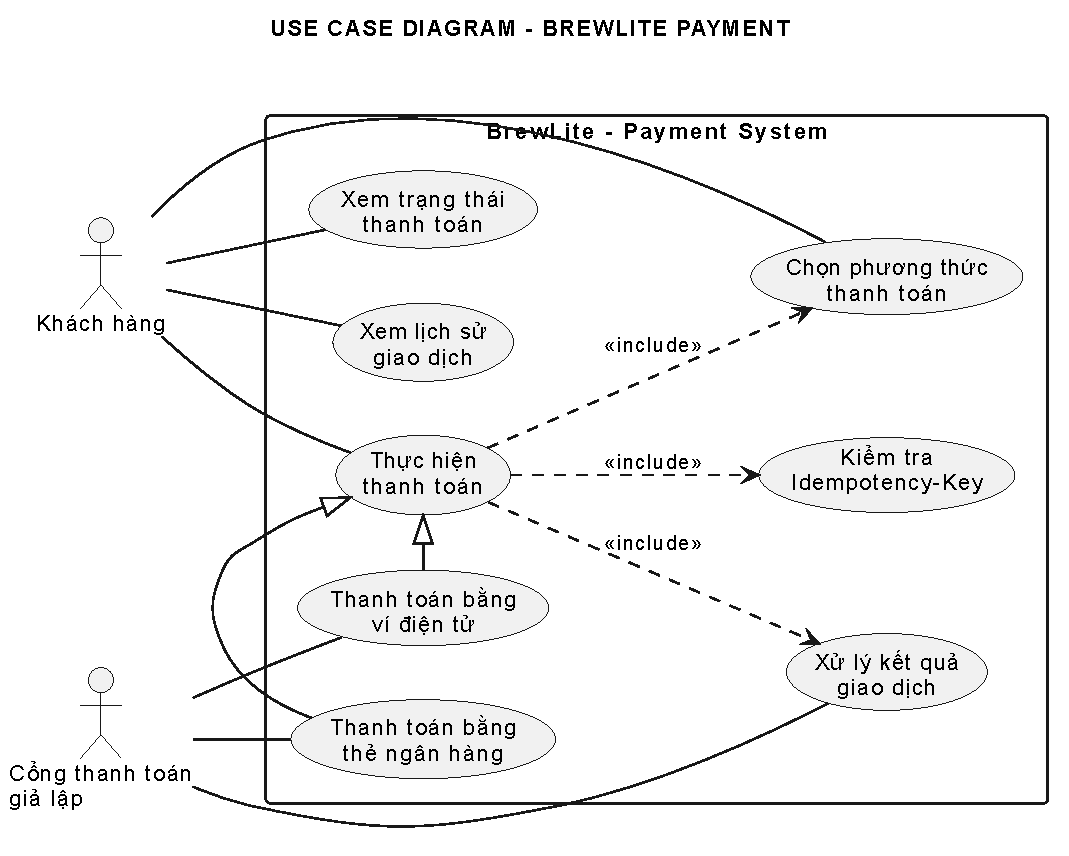
\includegraphics[width=0.75\textwidth]{figures/usecase-payment.pdf}
    \caption{Sơ đồ Use Case - Phân hệ Thanh toán}
    \label{fig:usecase-payment}
\end{figure}

\begin{table}[H]
\centering
\small
\caption{Đặc tả Use Case: Thực hiện Thanh toán Trực tuyến (UC-PAY-01)}
\label{tab:uc-spec-payment}
\begin{tabularx}{\textwidth}{p{2.8cm}X}
\toprule
\textbf{Mục} & \textbf{Chi tiết Đặc tả} \\
\midrule
\textbf{Actor} & Khách hàng đã đăng nhập, Cổng thanh toán giả lập (Mock Gateway) \\
\midrule
\textbf{Tiền điều kiện} & Đơn hàng tồn tại ở trạng thái \texttt{PENDING}; chưa được thanh toán thành công. \\
\midrule
\textbf{Hậu điều kiện} & Bản ghi thanh toán được lưu trữ; trạng thái đơn hàng chuyển thành \texttt{PAID}; điểm loyalty được cộng vào tài khoản khách hàng. \\
\midrule
\textbf{Luồng chính} & 
1. Khách hàng truy cập trang thanh toán \texttt{/payment/[orderId]}.\newline
2. Chọn phương thức thanh toán: Thẻ ngân hàng (\texttt{BANK\_CARD}) hoặc Ví điện tử (\texttt{E\_WALLET}).\newline
3. Nhấn "Thanh toán ngay".\newline
4. Trình duyệt tự động sinh mã UUID \texttt{Idempotency-Key} duy nhất và gửi request \texttt{POST /api/v1/payments}.\newline
5. PaymentsService kiểm tra \texttt{idempotencyKey}:\newline
\quad a. Nếu khóa đã tồn tại trong DB: Gọi \texttt{replayExistingPayment()} đối chiếu mã băm SHA-256 trên \texttt{\{orderId, method\}}. Nếu trùng khớp, trả lại kết quả đã lưu mà không gọi lại Mock Gateway; nếu sai lệch tải trọng, ném ngoại lệ \texttt{409 Conflict}.\newline
\quad b. Nếu là khóa mới: Khởi tạo giao dịch \texttt{payments} trong \texttt{prisma.\$transaction} với trạng thái \texttt{PENDING} và lưu mã băm \texttt{requestHash}.\newline
\quad c. Xử lý tranh chấp đồng thời: Nếu hai request cùng gửi một khóa, lỗi trùng khóa Unique (\texttt{P2002}) được bắt trong khối \texttt{catch}, tự động truy vấn lại giao dịch vừa tạo và phát lại (\textit{replay}) kết quả an toàn.\newline
6. Backend gọi Mock Payment Gateway để xác thực giao dịch.\newline
7. Khi Gateway phản hồi thành công (\texttt{SUCCESS}):\newline
\quad a. Cập nhật bản ghi \texttt{payments} thành \texttt{SUCCESS} kèm \texttt{transactionRef}.\newline
\quad b. Cập nhật đơn hàng: \texttt{status = PAID}, \texttt{paidAt = NOW()}.\newline
\quad c. Cộng điểm tích lũy mới vào \texttt{users.loyalty\_points}.\newline
\quad d. Ghi nhận giao dịch cộng điểm vào \texttt{loyalty\_transactions} (type: \texttt{EARNED}).\newline
\quad e. Ghi nhật ký vào \texttt{order\_status\_history} (PENDING \(\to\) PAID).\newline
8. Giao diện thông báo thanh toán thành công và điều hướng sang trang Lịch sử đơn hàng. \\
\midrule
\textbf{Luồng ngoại lệ} & 
- Gateway từ chối hoặc giao dịch thất bại: Cập nhật bản ghi payment thành \texttt{FAILED}, đơn hàng chuyển sang \texttt{PAYMENT\_FAILED}, cho phép khách hàng nhấn thử lại (tạo lượt payment mới).\newline
- Đơn hàng đã được thanh toán trước đó: Báo lỗi \texttt{400 Bad Request} ("Đơn hàng đã được thanh toán").\newline
- Trùng Idempotency-Key nhưng khác payload: Báo lỗi \texttt{409 Conflict} (\"Idempotency-Key đã được sử dụng với nội dung khác\"). \\
\bottomrule
\end{tabularx}
\end{table}

\clearpage
\subsection{Sơ đồ Hoạt động (Activity Diagram)}
Quy trình thẩm định Idempotency, gọi cổng thanh toán và xử lý kết quả giao dịch được mô tả tại Hình~\ref{fig:activity-payment}.

\begin{figure}[H]
    \centering
    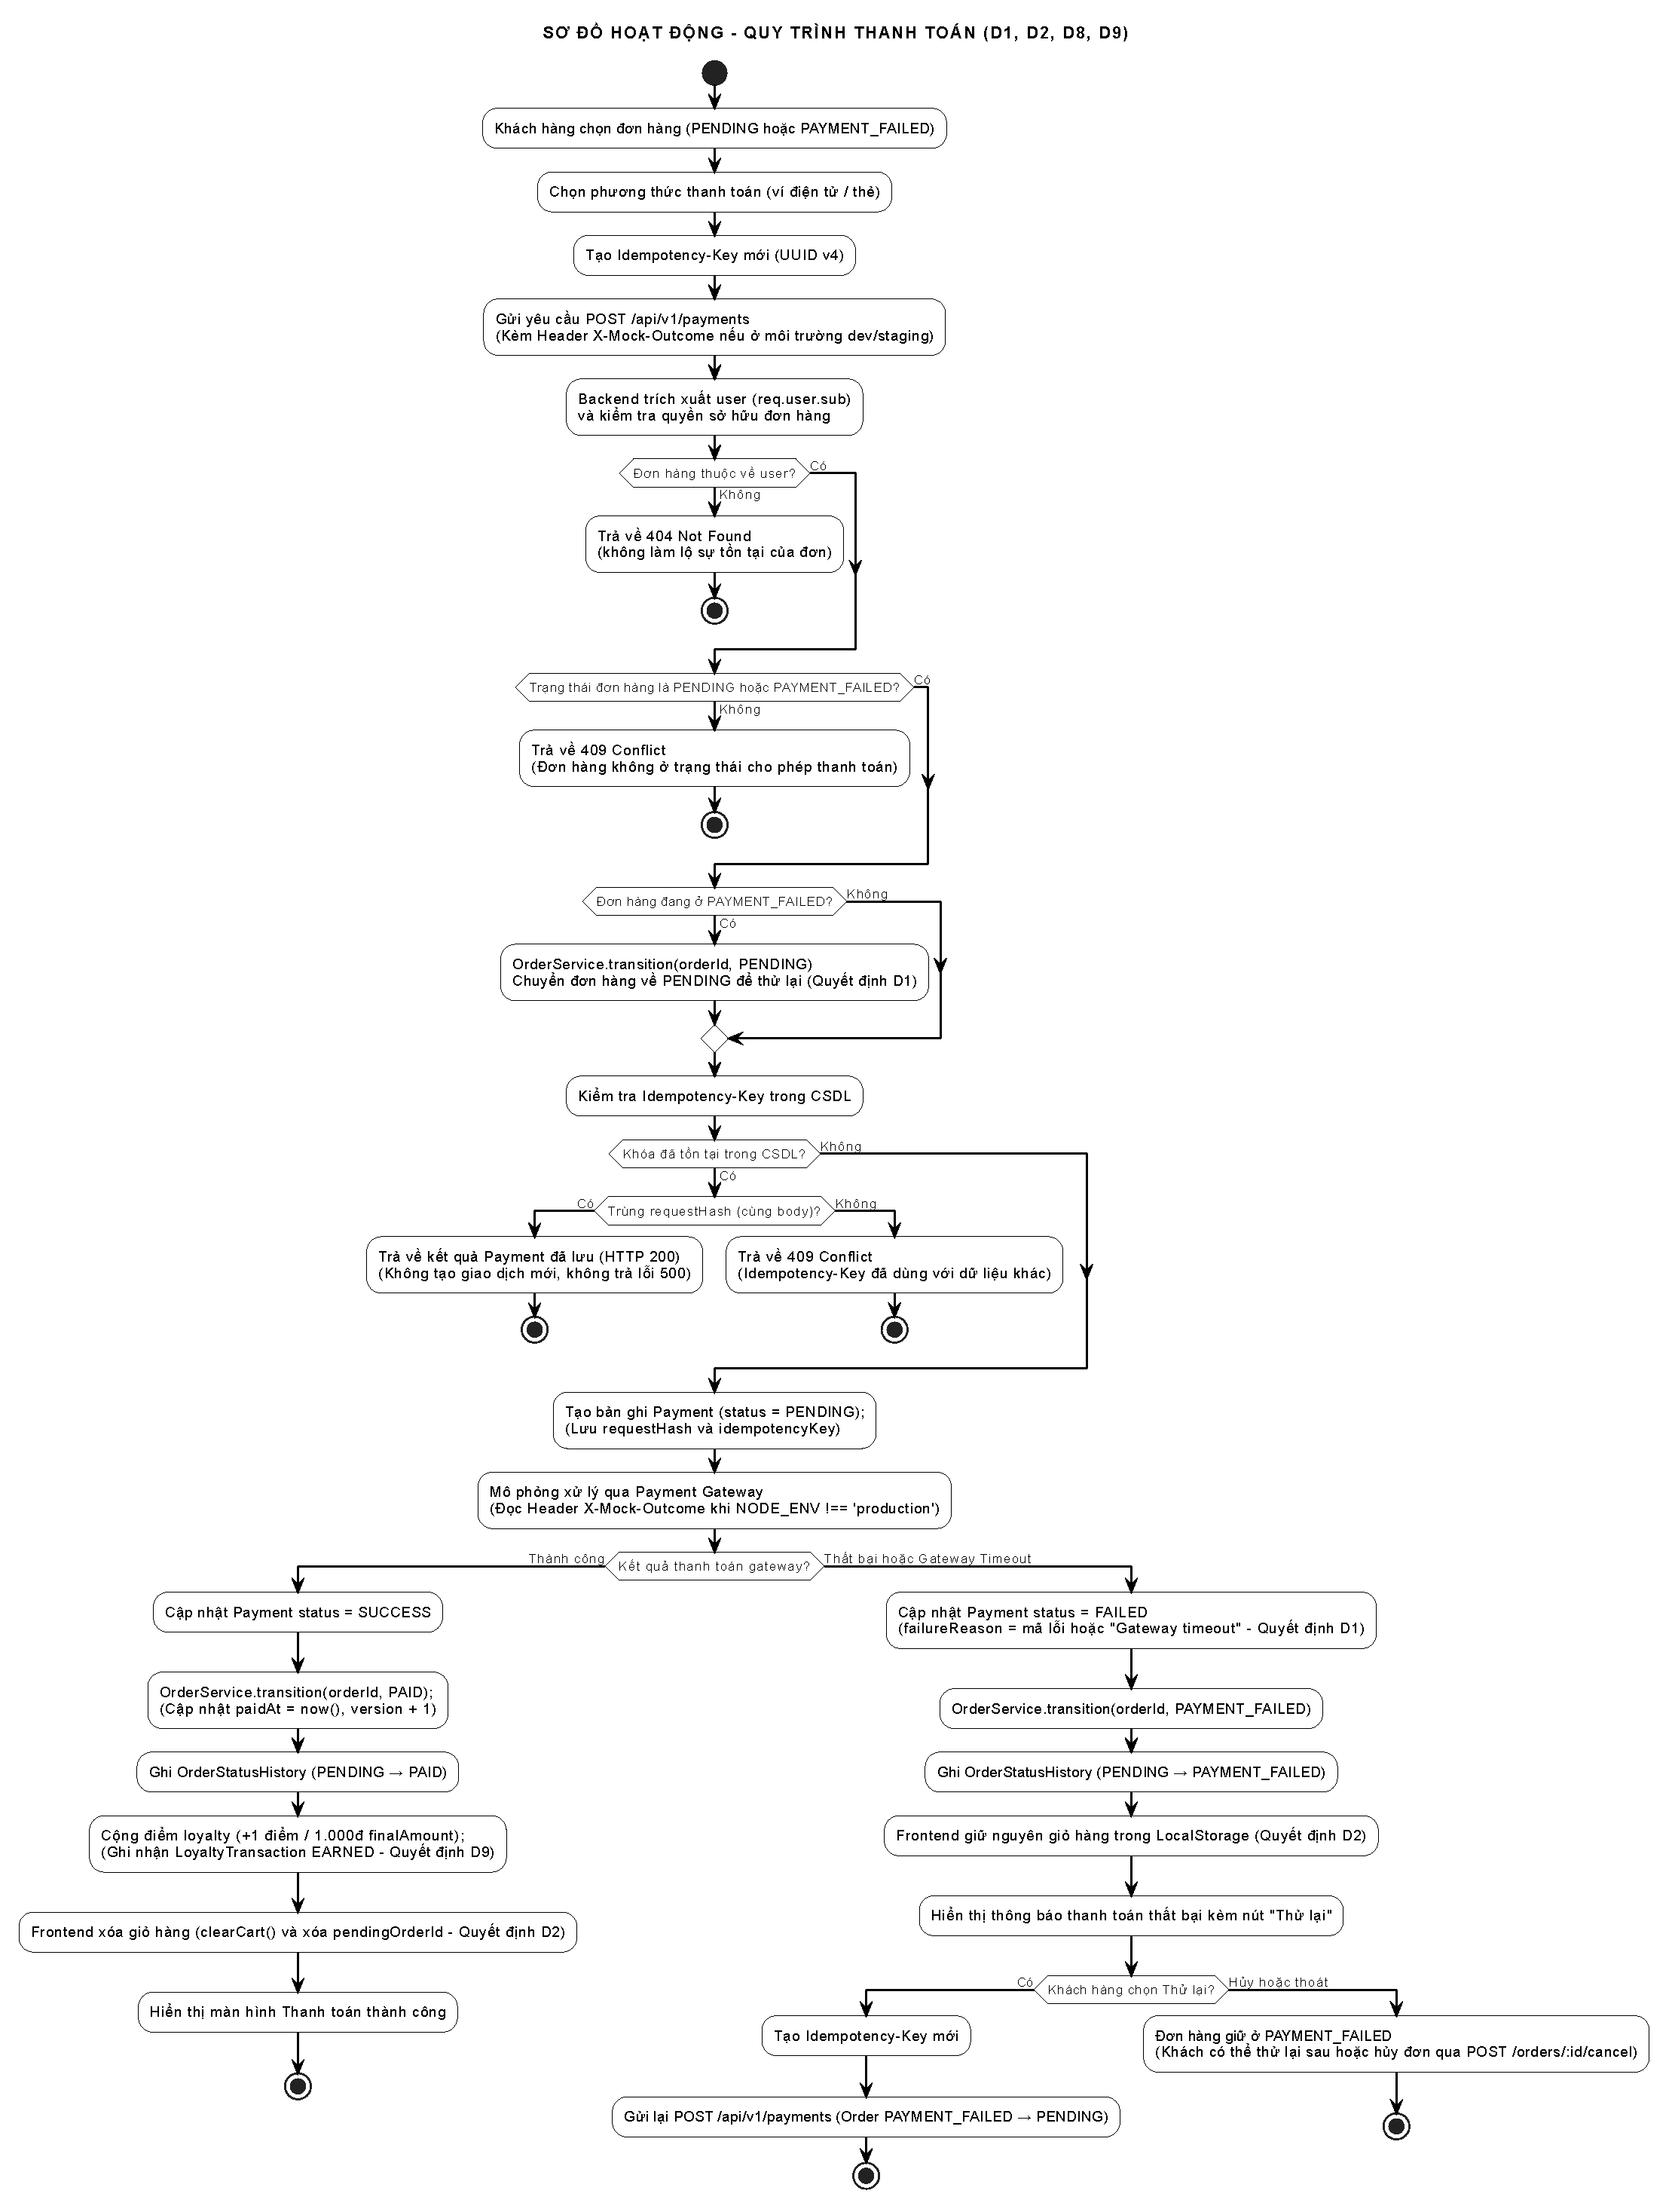
\includegraphics[width=\textwidth, height=0.80\textheight, keepaspectratio]{figures/activity-payment.pdf}
    \caption{Sơ đồ Hoạt động - Phân hệ Thanh toán}
    \label{fig:activity-payment}
\end{figure}

\clearpage
\subsection{Sơ đồ Tuần tự (Sequence Diagram)}
Sơ đồ Tuần tự phản ánh toàn diện các luồng tương tác giữa Frontend, PaymentsController, PaymentsService, Prisma DB và Mock Payment Gateway tại Hình~\ref{fig:sequence-payment}.

\begin{figure}[H]
    \centering
    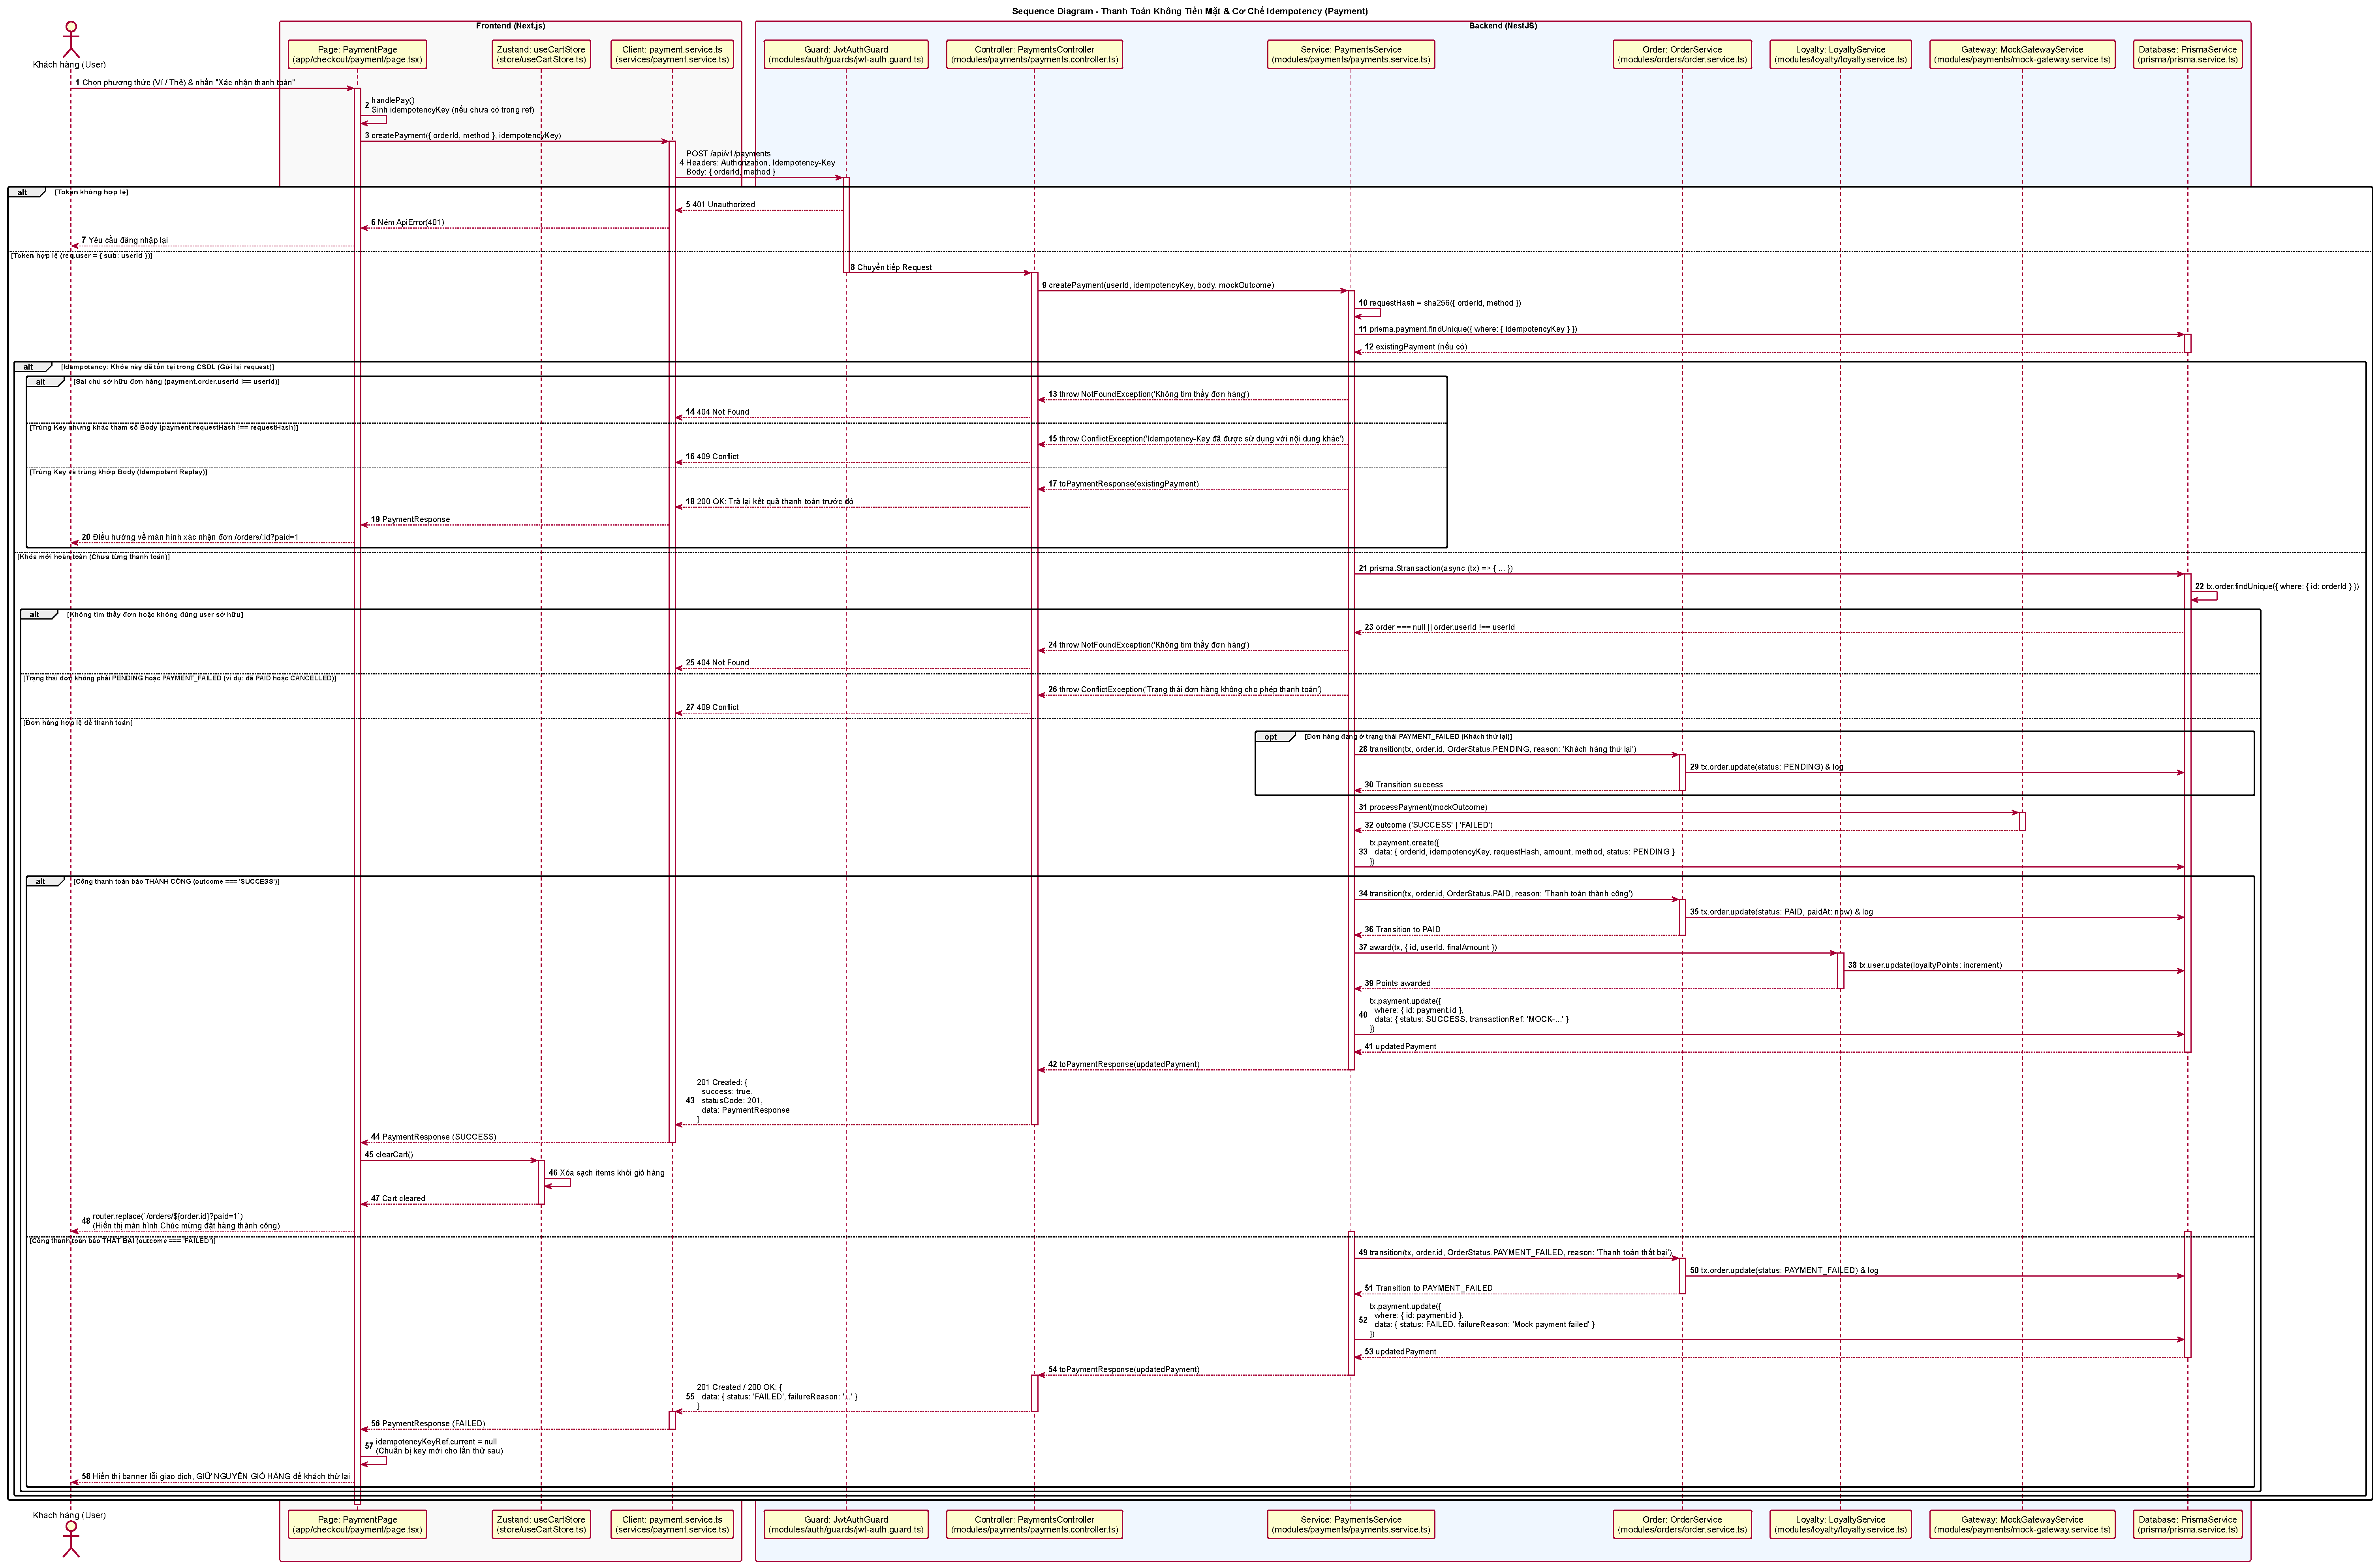
\includegraphics[width=\textwidth, height=0.80\textheight, keepaspectratio]{figures/sequence-payment.pdf}
    \caption{Sơ đồ Tuần tự - Phân hệ Thanh toán (Idempotent Flow \& Gateway Integration)}
    \label{fig:sequence-payment}
\end{figure}

\clearpage
\subsection{Hợp đồng API (API Contract)}
\begin{table}[H]
\centering
\small
\caption{Danh mục API Endpoints - Phân hệ Thanh toán}
\label{tab:api-payment}
\begin{tabularx}{\textwidth}{llp{4.5cm}X}
\toprule
\textbf{Phương thức} & \textbf{Endpoint} & \textbf{Headers \& Body} & \textbf{Phản hồi chính} \\
\midrule
\texttt{POST} & \texttt{/api/v1/payments} & 
Header: \texttt{Idempotency-Key: <UUID>}, Bearer Token.\newline Body: \texttt{\{orderId, method\}} & 
\texttt{200 OK}: Trả về chi tiết thanh toán thành công (hoặc kết quả phát lại). Lỗi: \texttt{400 Bad Request}, \texttt{401 Unauthorized}, \texttt{404 Not Found}, \texttt{409 Conflict} (sai lệch requestHash hoặc trạng thái đơn không hợp lệ). \\
\texttt{GET} & \texttt{/api/v1/payments/:id} & Tham số \texttt{id} bản ghi thanh toán & 
\texttt{200 OK}: Tra cứu trạng thái giao dịch thanh toán hiện tại. \\
\bottomrule
\end{tabularx}
\end{table}

\subsection{Ánh xạ Cơ sở dữ liệu (Database Mapping)}
\begin{itemize}
    \item \textbf{Cơ chế Idempotency:} Bảng \texttt{payments} sử dụng ràng buộc \texttt{@unique} trên trường \texttt{idempotency\_key} kết hợp cùng \texttt{request\_hash} sinh từ thuật toán SHA-256 trên nội dung JSON của body request:
    \begin{lstlisting}[language=SQL]
SELECT id, status, request_hash, transaction_ref 
FROM payments 
WHERE idempotency_key = :idempotencyKey;
    \end{lstlisting}
    \item \textbf{Cập nhật sau thanh toán thành công:} Thực thi trong transaction cập nhật đồng thời 4 bảng:
    \begin{lstlisting}[language=SQL]
UPDATE payments SET status = 'SUCCESS', transaction_ref = :ref WHERE id = :paymentId;
UPDATE orders SET status = 'PAID', paid_at = NOW() WHERE id = :orderId;
UPDATE users SET loyalty_points = loyalty_points + :pointsEarned WHERE id = :userId;
INSERT INTO loyalty_transactions (id, user_id, order_id, points, type, reason, created_at)
VALUES (cuid(), :userId, :orderId, :pointsEarned, 'EARNED', 'Tich diem tu don hang', NOW());
INSERT INTO order_status_history (id, order_id, from_status, to_status, changed_by, created_at)
VALUES (cuid(), :orderId, 'PENDING', 'PAID', 'payment_gateway', NOW());
    \end{lstlisting}
\end{itemize}

\subsection{Kịch bản Kiểm thử (Test Cases)}
\begin{table}[H]
\centering
\small
\caption{Tóm lược các Ca kiểm thử tiêu biểu - Phân hệ Thanh toán}
\label{tab:tc-payment}
\begin{tabularx}{\textwidth}{llp{2.6cm}p{3cm}Xc}
\toprule
\textbf{Mã TC} & \textbf{Loại} & \textbf{Tiền điều kiện} & \textbf{Endpoint / Màn hình} & \textbf{Kết quả mong đợi} & \textbf{Trạng thái} \\
\midrule
\texttt{TC-PAY-API-01} & Hợp lệ & Đơn PENDING, key mới & \texttt{POST /payments} & HTTP 200, status SUCCESS, đơn chuyển sang PAID & Chưa chạy \\
\texttt{TC-PAY-API-03} & Idempotent & Gửi lại cùng key & \texttt{POST /payments} & HTTP 200, trả về kết quả cũ, không gọi lại gateway & Chưa chạy \\
\texttt{TC-PAY-API-05} & Lỗi & Đơn đã thanh toán & \texttt{POST /payments} & HTTP 400, báo lỗi đơn hàng đã thanh toán & Chưa chạy \\
\texttt{TC-PAY-UI-01} & Giao diện & Đơn hàng chờ & Trang \texttt{/payment/[id]} & Hiển thị tổng tiền và 2 phương thức thẻ/ví & Chưa chạy \\
\bottomrule
\end{tabularx}
\end{table}

\subsection{Giao diện Người dùng}
\begin{figure}[H]
    \centering
    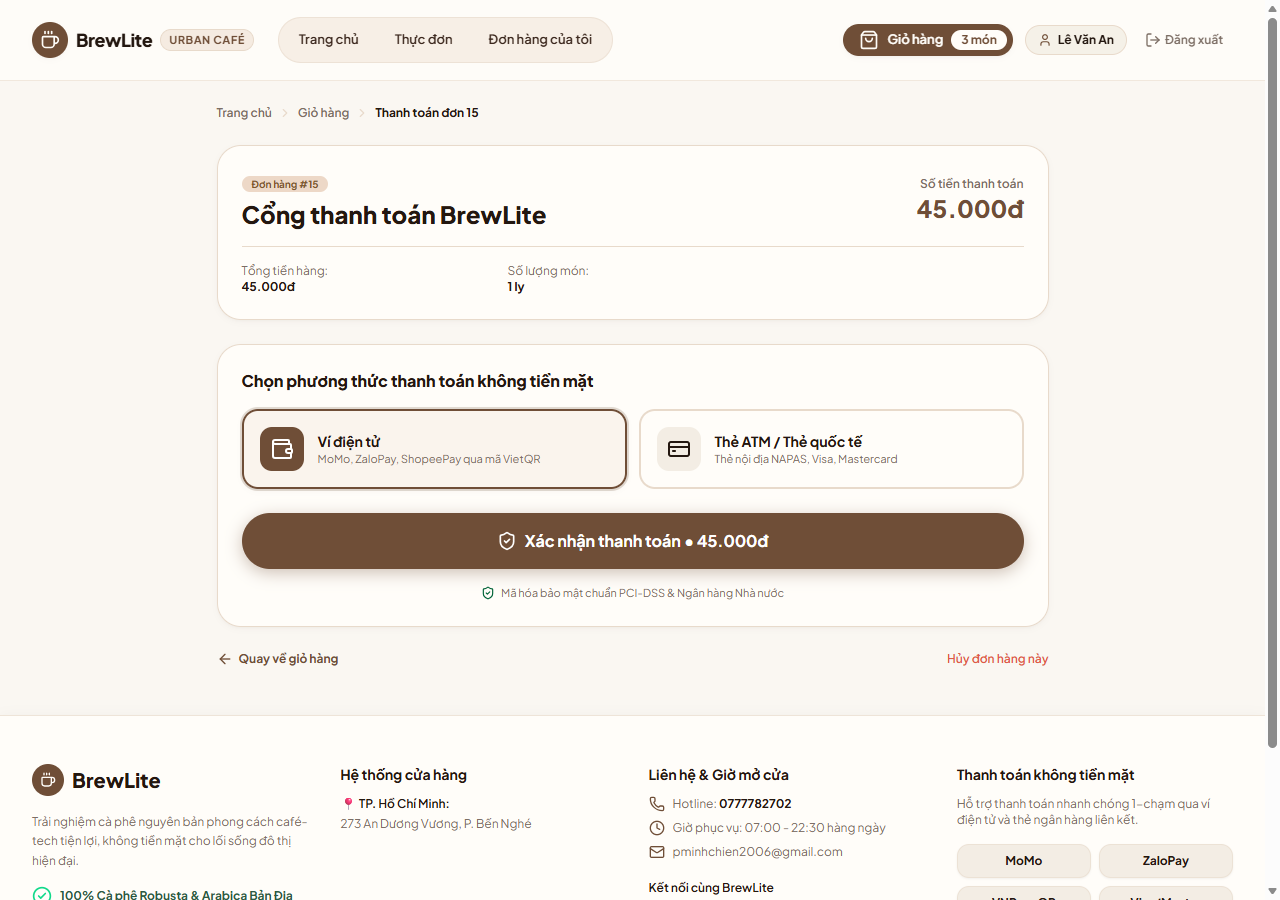
\includegraphics[width=0.92\textwidth]{figures/ui-payment.png}
    \caption{Giao diện Cổng thanh toán không tiền mặt đa phương thức}
    \label{fig:ui-payment}
\end{figure}
